\section{Quantum Physics}
    \subsection{Light: Particle and wave model}
        \textbf{Wave model}: double slit experiment. Light has properties of wave.

        \textbf{Particle model}: photoelectric effect. Light emit to matal and electrons emit from metal. 
    
    \subsection{Photoelectric effect}
        Light of specific range of frequency light on a metal plate and the plate emit electrons.

        \begin{figure}[H]
            \begin{center}
                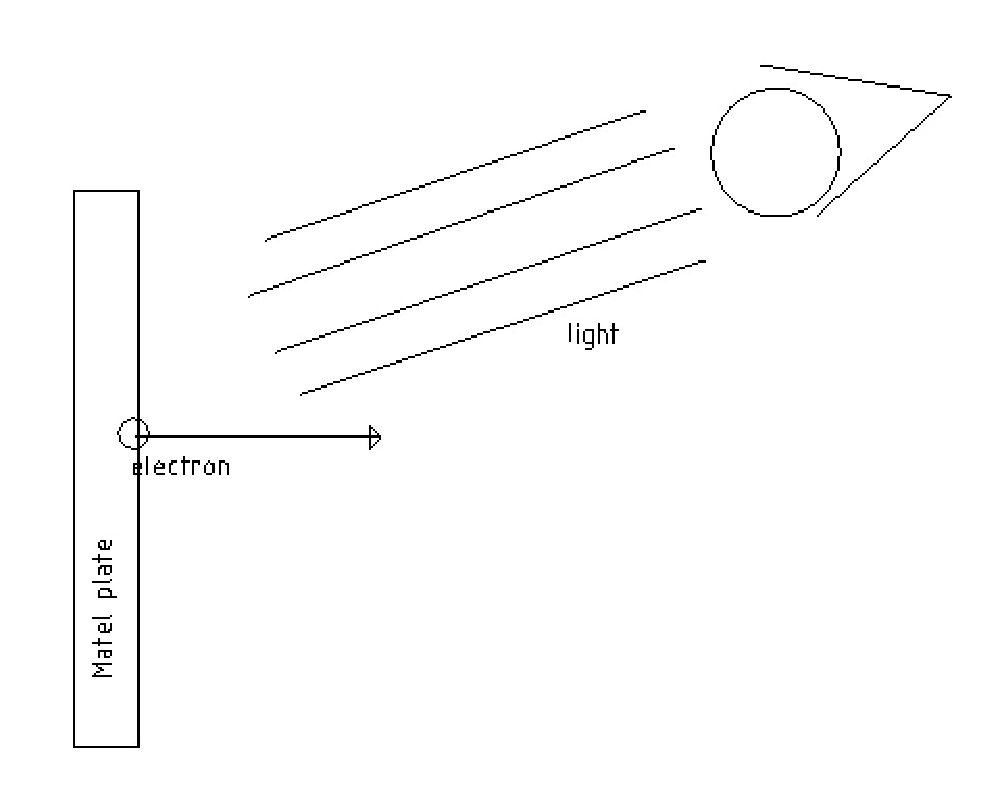
\includegraphics[height=5cm]{quantum_charts/photo_ele_show.eps}
            \end{center}
            \caption{Diagram of photoelectric effect experiment}
            \label{pe_exp_dia}
        \end{figure}

        \paragraph{Why photoelectric effect can not be explained with wave model}
            \begin{enumerate}
                \item For light with low frequency (which means low energy per photon), electrons can not emit even with long time lighting.
                        This shows energy of light can not accumulate on the electrons. 
                \item There is not time delay for electrons to emit.
                        If light is wave, it need time to transfer enough energy to emit the electrons. If light is particle, it has energy itself and can transfer its energy to electrons as it hit the electrons with no delay.
            \end{enumerate}
        
        \paragraph{Work function}
            Work function, $\phi$, is the energy required for the electron transit to ground state. It depends on the material. 

        \paragraph{Threshold frequency}
            Threshold frequency is the minimum frequency of light that can emit electrons.

            The energy of a photon with frequency $f$ is $E_p = hf$. When $E_p > \phi$, the electron emit. Thus the threshold frequency is
            \begin{align}
                f_{min} = \frac{\phi}{h}
            \end{align}

        \paragraph{Kinetic energy of emitted electron}
            Some energy of photon is used for the electrons to transit to ground state. The rest energy turns to electrons' kinetic energy. Thus the kinetic energy of the emitted electron is
            \begin{align}
                E_k = hf - \phi
            \end{align}

            This function is shown in Figure \ref{thres_freq_func}

            \begin{figure}[H]
                \begin{center}
                    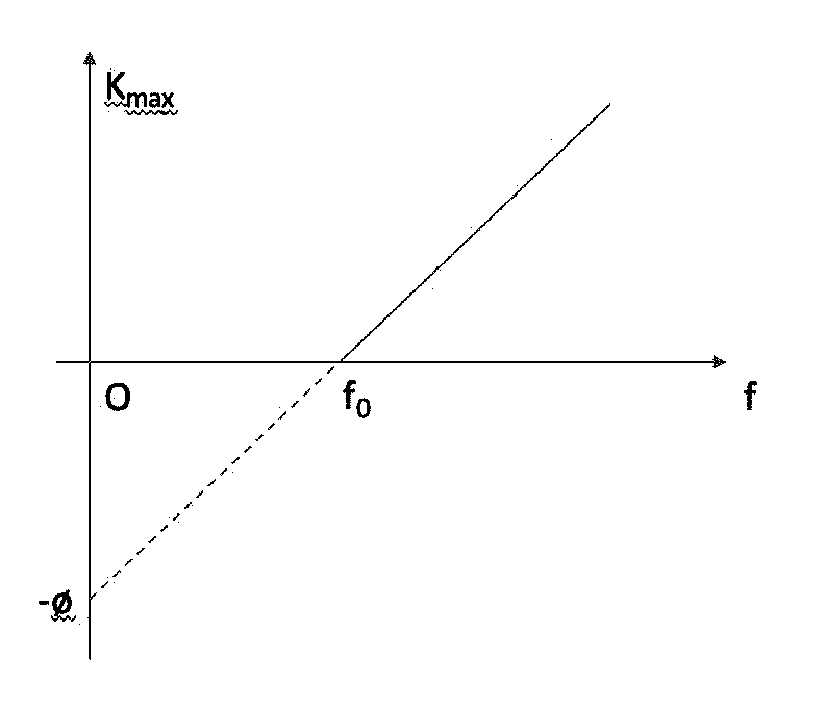
\includegraphics[height=5cm]{quantum_charts/thres_freq_func.eps}
                \end{center}
                \caption{Kinetic energy against frequency}
                \label{thres_freq_func}
            \end{figure}

        \paragraph{Photoelectric in circuit}
            Figure \ref{ph_ele_in_circ} shows a photoelectric pannel serial connected in a circuit with a cell and an ampere meter. 

            \begin{figure}[H]
                \begin{center}
                    \includegraphics[height=7cm]{quantum_charts/photo_ele_in_circ.eps}
                \end{center}
                \caption{Photoelectric experiment in circuit}
                \label{ph_ele_in_circ}
            \end{figure}

            With cell voltage $U$, the energy required for the electron to emit is $\phi + eU$ \footnote{[$e$]: amount of charge of one electron, $e = 1.6 \times 10^{-19} \mathrm{C}$}. Thus the threshold frequency is $\frac{\phi + eU}{h}$.

            Stop voltage, $U_0$, is when the voltage of cell that the electrons just can not emit. It is calculated by
            \begin{align}
                &\phi + eU = hf \\
                &\Rightarrow U = \frac{hf - \phi}{e}
            \end{align}

            The current in the circuit, $I$, can be calculated by
            \begin{align}
                I &= \frac{Q}{t} \\
                    &= \frac{eN}{t} \\
            \end{align}

            Here $N$ is the number of photons per second.
        
        \paragraph{Relation to the intensity of light}
            Defination of intensity: energy radiated per unit area.
            \begin{align}
                I = \frac{P}{A}
            \end{align}

            Thus, intensity of light is
            \begin{align}
                I &= \frac{P}{A} \\
                    &= \frac{\frac{N h f}{t}}{A} \\
                    &= \frac{N h f}{A t}
            \end{align}

            Thus number of photons emitted per second is
            \begin{align}
                N = \frac{I A t}{h f}
            \end{align}

            Thus, with same intensity, the higher frequency is, the smaller number of photons emitted. Photon and electron is one-to-one. Thus higher frequency is, lower current in the circuit.

    \subsection{Mass wave}
        \paragraph{Davisson Germer experiment}
            \begin{figure}[H]
                \begin{center}
                    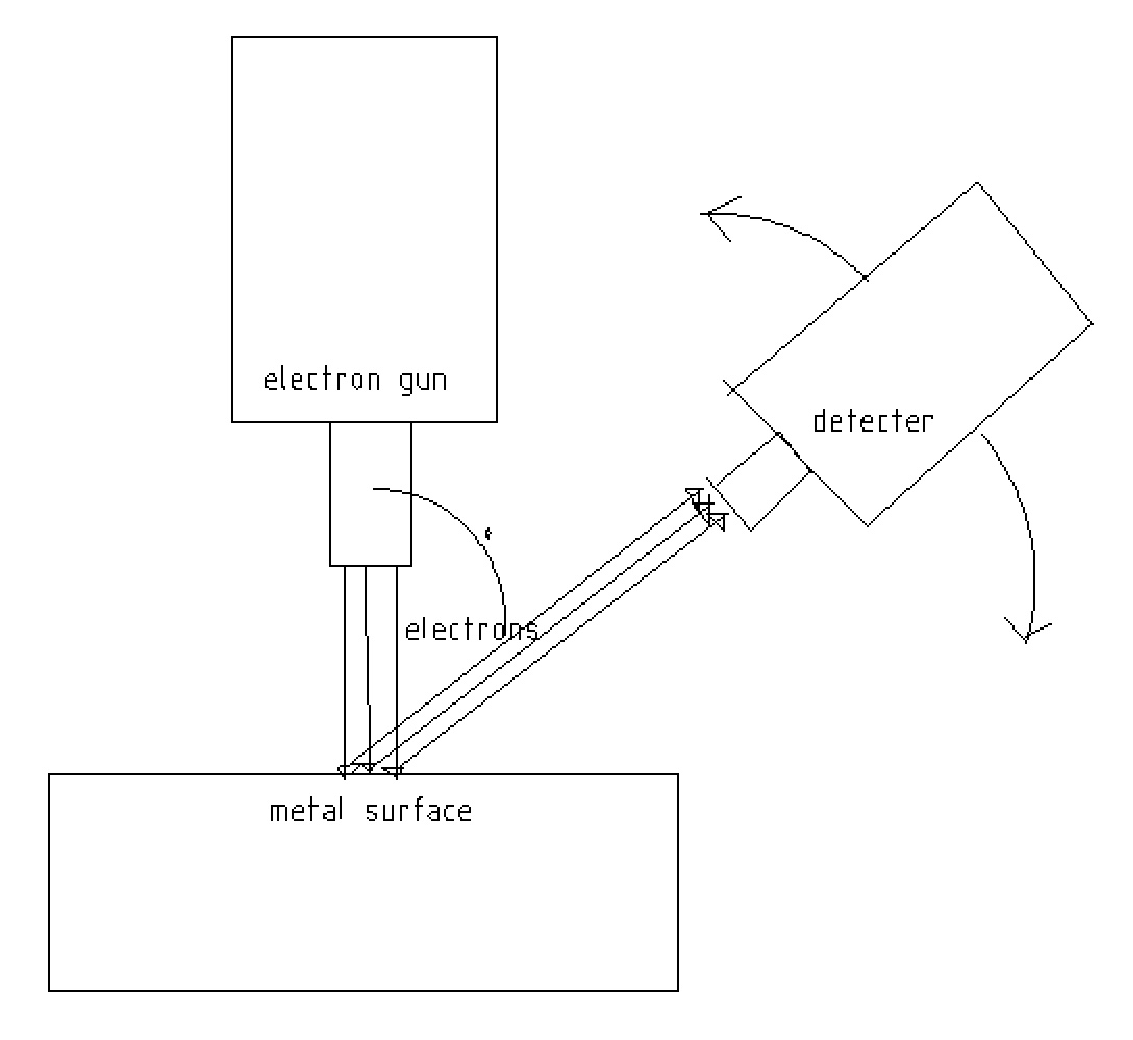
\includegraphics[height=5cm]{quantum_charts/dav_germ_exp.eps}
                \end{center}
                \caption{Davisson Germer experiment}
                \label{dav_germ_exp}
            \end{figure}

            In this experiment, change the angle between incident electrons and detecter, the intensity of electrons detected change with partern same as diffraction partern.

            This is because the electrons are diffracted by the metal lattice. This shows electrons have properties of wave.

        \paragraph{De Broglie Wave}
            De Broglie found that matter is wave. It shows probability of the position of matter. De Broglie wave length is
            \begin{align}
                \lambda = \frac{h}{p}
            \end{align}

            $h$ is the Plank constant, $p$ is the momentum of the matter.

    \subsection{Bohr model}
        \paragraph{Energy of electron}
            The kinetic energy of spinning electron is
            \begin{align}
                & m \frac{v^2}{r} = k \frac{e^2}{r^2} \\
                & \Rightarrow v = \sqrt{\frac{k e^2}{m r}} \\
                & \Rightarrow E_k = \frac{1}{2} m v^2 = \frac{k e^2}{2 r}
            \end{align}

            Thus, total energy of electron is
            \begin{align}
                E_T &= E_k + E_p  \\
                    &= - k \frac{e^2}{r} + \frac{k e^2}{2 r} \\
                    &= -k \frac{e^2}{2 r}
                \label{eqn_ele_ke}
            \end{align}

            Electron spin around the nucleus has angular momentum. It is
            \begin{align}
                L &= m v r \\ 
                  &=n \frac{h}{2 \pi}\ , \ n \in Z^+
                \label{eqn_ang_p}
            \end{align}

            From Equation \ref{eqn_ele_ke} and Equation \ref{eqn_ang_p}, the possible energy of electron is
            \begin{align}
                E &= -k \frac{e^2}{2 \frac{n h}{2 \pi m v}} \\
                  &= - \frac{\pi m v }{n h} k e^2\ , \ n \in Z^+
            \end{align}
        
        \paragraph{Electron cloud}
            Electron is a "cloud" that it randomly appears in somewhere by possibility. 

        \paragraph{Model for $_1^1 H$}
            Restriction of Bohr's model is only applicable for atom of one-proton-one-electron, which is $_1^1 H$.

            % Partern of electron:
            % \begin{align}
            %     & \left\{
            %         \begin{aligned}
            %             & L = m v r = pr \\
            %             & L = \frac{n h}{2 \pi}
            %         \end{aligned}
            %     \right. \Rightarrow 
            %     r = \frac{n}{2 \pi} \frac{h}{p} \\
            %     & \because \lambda = \frac{h}{p} \\
            %     & \therefore r = \frac{n}{2 \pi} \lambda \\
            %     & \therefore c = 2 \pi r = n \lambda
            % \end{align}

            Speed of orbiting electron
            \begin{align}
                & \frac{k e^2}{r^2} = m \frac{v^2}{r} \Rightarrow r = \frac{k e^2}{m v^2} \\
                & m v r = \frac{n h}{2 \pi} \Rightarrow r = \frac{n h}{2 \pi m v} \\
                & \therefore \frac{n h}{2 \pi m v} = \frac{k e^2}{m v^2} \\
                & \therefore v = \frac{2 \pi k e^2}{n h} \ , \ n \in Z^+
            \end{align}


        
        \paragraph{Energy state of electrons in $_1^1 H$}
            \begin{align}
                E_T = - E_k &= - \frac{1}{2} m v^2 \\
                            &= - \frac{1}{2} m (\frac{2 \pi k e^2}{n h})^2 \\
                            &= - \frac{2 \pi^2 m k^2 e^4}{n^2 h^2} \ , \ n \in Z^+
                \label{eqn_ele_ene_stat}
            \end{align}

            Substitude constants into Equation \ref{eqn_ele_ene_stat}, the energy state of electron in $_1^1 H$ is
            \begin{align}
                E = - \frac{13.6}{n^2} \mathrm{ev} \ , \ n \in Z^+
            \end{align}

    \subsection{Wave function}
        Wave function show the probability of the position of the electron.
        Wave function of electron in $_1^1 H$:
        \begin{align}
            i h \frac{\partial \Psi}{\partial t} = -\frac{h^2}{2 m} \frac{\partial^2 \Psi}{\partial x^2} + V \Psi
        \end{align}

        Probability for the electron to be at position $x$ at time $t$:
        \begin{align}
            P(x, t) = | [\Psi(x, t)]^2| \Delta V 
        \end{align}

        \paragraph{Position of particle before and after measurement}
            Before measurement the particle is at "Orthodox" position. It is at no where before measurement. The probability of position follows wave function.

            After measurement, the wave function collapse into a particular position.
    
    \subsection{Heisenberg uncertainty principle}
        \paragraph{Position and momentum uncertainty}
            \begin{align}
                \Delta x \Delta p \ge \frac{h}{4 \pi}
            \end{align}
            
            Here, $\Delta x$ is the uncertainty of position and $\Delta p$ is the uncertainty of momentum.
        
        \paragraph{Energy and time uncertainty}
            \begin{align}
                \Delta E \Delta t \ge \frac{h}{4 \pi}
            \end{align}

            Here, $\Delta E$ is the uncertainty of the energy state of the electron and $\Delta t$ is the time period that the electron remains in that state.
    
    \subsection{Tuning effect}
        Small mass have a probability to go across a potentio barrier without enough energy.

        \begin{figure}[H]
            \begin{center}
                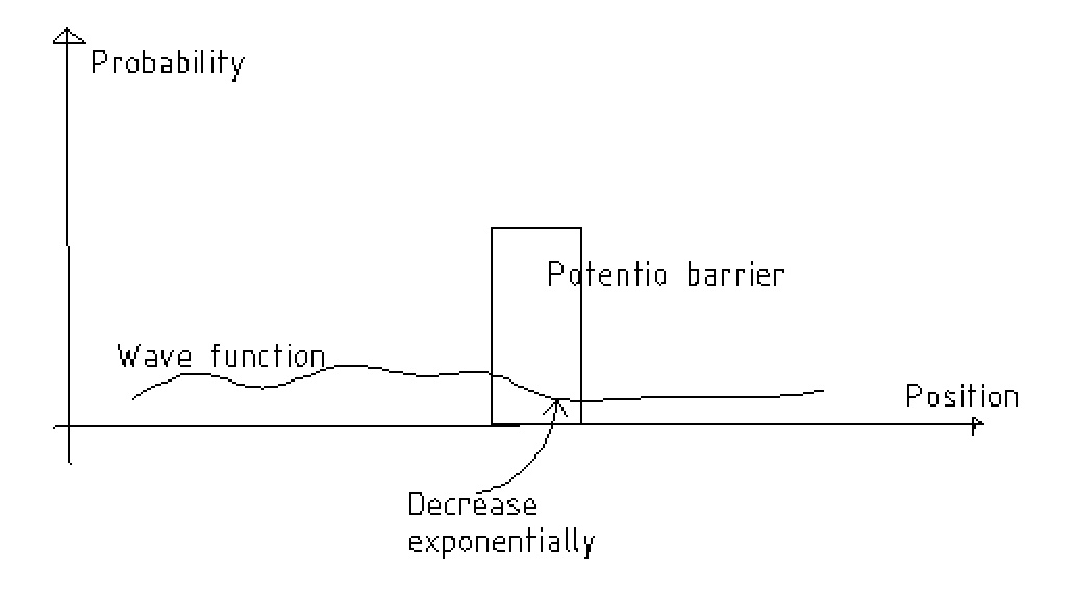
\includegraphics[height=5cm]{quantum_charts/tun_eff_prob.eps}
            \end{center}
            \caption{Probability of position with potentio barrier}
            \label{tun_eff_pppb}
        \end{figure}

        \paragraph{Factors that influence probability of tuning}
        \begin{enumerate}
            \item Mass of the particle
            \item Thickness of the barrier
            \item Height of the barrier
            \item Energy difference between particle and barrier 
        \end{enumerate}

        \paragraph{With uncertainty principle}
            For a particle with energy state $E_s$ trapped in a potential well with barrier of energy state $E_b$, the time that it be trapped in the well is
            \begin{align}
                \Delta t &= \frac{h}{4 \pi \Delta E} \\
                         &= \frac{h}{4 \pi (E_b - E_s)}
            \end{align}

        
        





            
            